\documentclass[twocolumn]{article} 

\usepackage[utf8]{inputenc} 
\usepackage[T1]{fontenc}    
\usepackage[english]{babel} 
\usepackage{amsmath}        
\usepackage{amssymb}        
\usepackage{amsfonts}       
\usepackage{graphicx}       
\usepackage{hyperref}       
\usepackage{geometry}       
\usepackage{enumitem}       
\usepackage{titling}
\usepackage{braket}
\usepackage{graphicx}
% \usepackage{multicol}
\usepackage{lipsum}

% Page layout
\geometry{margin=1cm}      
\geometry{bottom=2cm}
\geometry{top=0.5cm}
\setlength{\parindent}{0pt} 
\setlength{\parskip}{6pt}   % Space between paragraphs
% math commands
\newcommand{\Lagrange}{\mathcal{L}}
\newcommand{\Hamilton}{\mathcal{H}}
\newcommand{\deriv}[3][]{\frac{d^{#1} #2}{d #3^{#1}}}
\newcommand{\pderiv}[3][]{\frac{\partial^{#1} #2}{\partial #3^{#1}}}

\renewcommand{\labelenumii}{\theenumii}
\renewcommand{\theenumii}{\theenumi.\arabic{enumii}.}

\graphicspath{{../plots}}

\pretitle{\begin{center}\LARGE}
\posttitle{\par\end{center}\vskip 0.5em}

\title{Object Oriented, Multiprocessing Genetic Algorithm for N variable optimization}
\author{Alessandro Brovelli}
\date{\today}

\begin{document}

% Title
\twocolumn[
\begin{@twocolumnfalse}
\maketitle

% Abstract
\begin{abstract}
An object oriented genetic algorithm was developed in Python. 
The scope of the code is to optimize (maximize or minimize) a $N \geq 1$ variable fitness function in a provided search space.
It can employ a set of two selection, crossover and mutation methods, set by the user. The algorithm was tested on a 2 dimensional function (Styblinsky-Tang), for which parameters were tuned for optimal accuracy for each combination of evolutionary methods. To verify the stability around these optimized settings, a perturbative analysis was performed. Finally a speed test was carried out, to see how the different parameters affect the algorithm performance. 
\end{abstract}
\vspace{1em}
\end{@twocolumnfalse}
]

\section{Algorithm description}
\subsection{General structure}
The algorithm structure is divided in three classes. The first one, \textit{Individual}, defines a single candidate solution, expressed as a genome of N binary strings (\textit{chromosome}) of set length (\textit{number of genes}). Each chromosome can be decoded into a decimal value  the provided search space. The decoded genome will be the input of the N variable function used to evaluate the individual's fitness. Within itself, an individual can only mutate, given the mutation scheme and probability

A second class \textit{Population} establishes a candidate solutions population (a list of individuals), and contains a method to create it given size, number of chromosomes and genes per chromosome. The other methods in this class allow the population to breed with a certain crossover method and probability, and to mutate by iterating through the individuals.

The main class, \textit{Breeder}, inherits \textit{Population} and defines the settings and procedures of the genetic algorithm. It includes methods to decode each genome, evaluate the population's fitness and to select worthy individuals for breeding. By creating an object, the user can set the problem size and type (maximize or minimize) and the various selection, crossover and mutation parameters and methods, which will be explained in detail in the next section. The whole algorithm can be executed by calling the method \textit{start evolution}, which takes as input the fitness function, the search space, the error threshold and the generation number at which to stop if there is no convergence. If desired, at the end of the evolution the generational best fitness is plotted, alongside the fitness function in the search space with the final population scattered on it (if $N = 1$ or $N = 2$).

\subsection{Selection}
After evaluating the fitness of the current generation, the selection process begins. The aim is to choose the best individuals to reproduce, in order to evolve the population towards the optimal solution. Two selection methods are available: \textit{tournament} and \textit{entropy}. Each methods iterates through random batches of the population, in which an individual can be picked with set probability $ps$.

\textbf{Tournament}\\
A deterministic tournament selection method was employed. Only the individual with the best fitness is selected from each batch. This process is repeated until the selected population reaches the size of the initial one, which is therefore maintained constant through the generations.

\textbf{Entropy}\\
A more advanced selection is offered by the entropy method, inspired by simulated annealing optimization methods. Each individual in the current batch it is assigned a selection probability with the so called \textit{Metropolis criterion} \cite{EvComputing}, which for a minimization problem would be 
\begin{equation}
  \label{eq:Metropolis}
  P(i) = \begin{cases}
    1 \quad& F_i \leq F_{old}\\
    \exp\left(- \frac{\Delta F}{T}\right) \quad & F_i > F_{old}
  \end{cases}
\end{equation}
where $F_i$ fitness of $i^{th}$ individual, $F_{old}$ best fitness of previous generation and $\Delta F = |F_i - F_{old}|$. The parameter $T$ represents the \textit{temperature} and it decreases through the generations with an exponential trend
\begin{equation}
  T = T_0\; \alpha ^ n
  \label{eq:Temperature}
\end{equation}
where $T_0$ is the initial temperature, $n$ the generation number and \(0 < \alpha < 1\).
This method permits more exploration of the search space in the first genearations, when the temperature is higher, and more exploitation of the region where the solution will converge in the last generations. The selection iteration stops when the selected population reaches its former size or, to prevent being stuck in the loop when the temperature is too low, when a maximum number of batch evaluations is reached. This logic allows the population size to decrease through the generations, by letting unfit individuals to freeze.

\subsection{Crossover}
Amongst the selected population, pairs of parents are chosen at random to reproduce. With a set probability ($pc$) they will either generate a pair of children and die or live and be part of the next generation. Each children chromosome will be the combination of the two same chromosomes of the parents, with a specific crossover method. In \textit{one point} crossover the parents chromosomes are split at one random point, while in \textit{two point} crossover they are split in three at two random points. They are then recombined as shown in figure \ref{fig:1}

\begin{figure}[h]
  \begin{center}
    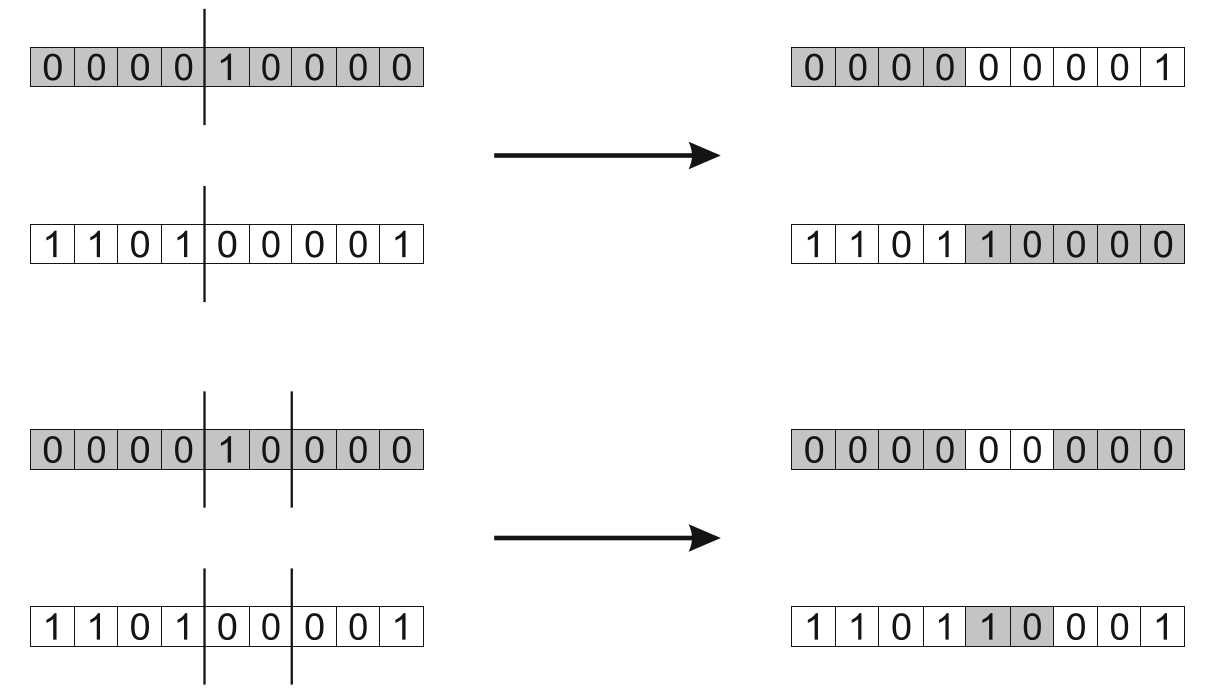
\includegraphics[width=0.45\textwidth]{crossover.png}
  \end{center} 
  \caption{Illustration of one point (top) and two point (bottom) crossover \cite{EvComputing}}\label{fig:1}
\end{figure}

\subsection{Mutation}
After the crossover, the children chromosomes can be mutated. This inserts a further random element in the evolution, allowing the population to explore the search space more efficiently and to prevent premature convergence.
The mutation probability ($pm$) is set by the user and it is the probability that a gene in the chromosome will be flipped. The mutation method can be either \textit{bit flip} or \textit{swap}. In the first case, a random gene is chosen and its value is inverted, while in the second case two random genes are swapped.

\section{Algorithm testing}
The algorithm was tested on the 2 dimensional Styblinsky-Tang function
\begin{equation}
  f(x, y) = \frac{1}{2} \left( x^4 - 16x^2 + 5x + y^4 - 16y^2 + 5y \right)
  \label{eq:Styblinsky-Tang}
\end{equation}
which has a global minimum at $f(-2.903534, -2.903534) = -78.3323$. The search space was \((x,y)\in[-5,5]\times[-5,5]\), the convergence threshold was set to $10^{-9}$ and the maximum number of generations at 500. The plot [] shows the result for VVV OPTIMAL SETTINGS.
These settings are the ones that give optimal accuracy for such combination of settings. They were found by tuning the algorithm, a procedure that will be described in the following section.

\section{Parametric analysis}

\subsection{Tuning with multiprocessing}
Tuning such an algorithm can be quite a time consuming task. For tournament selection, the total number of combinations of settings that can be tested are
\begin{equation}
  2^2\prod_{i=1}^5 n_i
  \label{eq:Tourn_settings_comb}
\end{equation}
where $2^2$ are the combinations of the 2 available crossover and mutation methods and $n_i$ are the lenghts of test parameter vectors which contain values of population size, number of genes and probabilities $ps$, $pc$ and $pm$. For entropy selection, the number of test vectors will be 7, considering also $T_0$ and $\alpha$.
To reduce the computational time for this process, parallel computing with multiprocessing was employed. Every combination of settings was tested once, and the most promising ones (error on the fitness function lower than $10^{-4}$) were retested 5 times. Only if every test yielded an error lower than the threshold, the settings were chosen as optimal.

\subsection{Perturbative test}
To verify the stability of the optimal settings, a perturbative analysis was carried out. The parameters were perturbed randomly with various maximum amplitudes, and the best fitness was recorded for each test. To speed up the process, multiprocessing was used here as well.  VVV PLOTS AND STABILITY CONSIDERATIONS

\subsection{Speed test}

\section{Conclusions and future developments}


\bibliographystyle{plain}
\bibliography{ref}

\end{document}
